\chapter{Simple Network Management Protocol}\label{ch:snmp}
Large networks has too many components to be managed by human agents alone. Network devices have to maintain a large amount of management data such as configuration information,  operational state and statistics. Management information can be used to understand how a network performs, how devices in a network are configured and to change their configuration. The Simple Network Management Protocol (SNMP) \cite{rfc3410} is an application layer protocol that facilitates the exchange of management information between network devices. It exposes management data in the form of variables on the managed systems, which describe the system configuration. Since its first publication in 1988, the SNMP protocol has become the most widely-used network management tool for IP-based networks.

Currently, there are three versions of SNMP defined. The first version (SNMPv1) is nowadays a historical IETF standard, although it is still widely supported by many vendors. SNMPv1 has been criticized for its poor security based on a community string, which is a type of password transmitted in cleartext. SNMPv2 extended the functionality of SNMPv1 and includes a number of improvements, such as additional protocol operations. A new security system was proposed, however, it was too complex and was not widely accepted. SNMPv3 addresses the security problems of the previous versions. The SNMPv3 architecture introduces a well defined extensible architecture and the User-based Security Model (USM) for message security.

The SNMP protocol is datagram-oriented and its implementation can be very lightweight \cite{draft-6lowpan-snmp}. It can fit resource-constrained devices very well. This makes it a perfect candidate as a management protocol for 6LoWPAN applications. In this chapter an overview of the SNMP protocol is given.

\section{Protocol Architecture}
The SNMP protocol consists of four basic components: an entity which provides remote access to management instrumentation (typically called as an agent); an entity running management applications (typically called a manager); a management protocol to convey management information between the entities; and management information.

According to the SNMP architecture \cite{rfc3411}, an SNMP entity consists of an SNMP engine and one or more associated applications.

\begin{figure}	
\begin{center}
    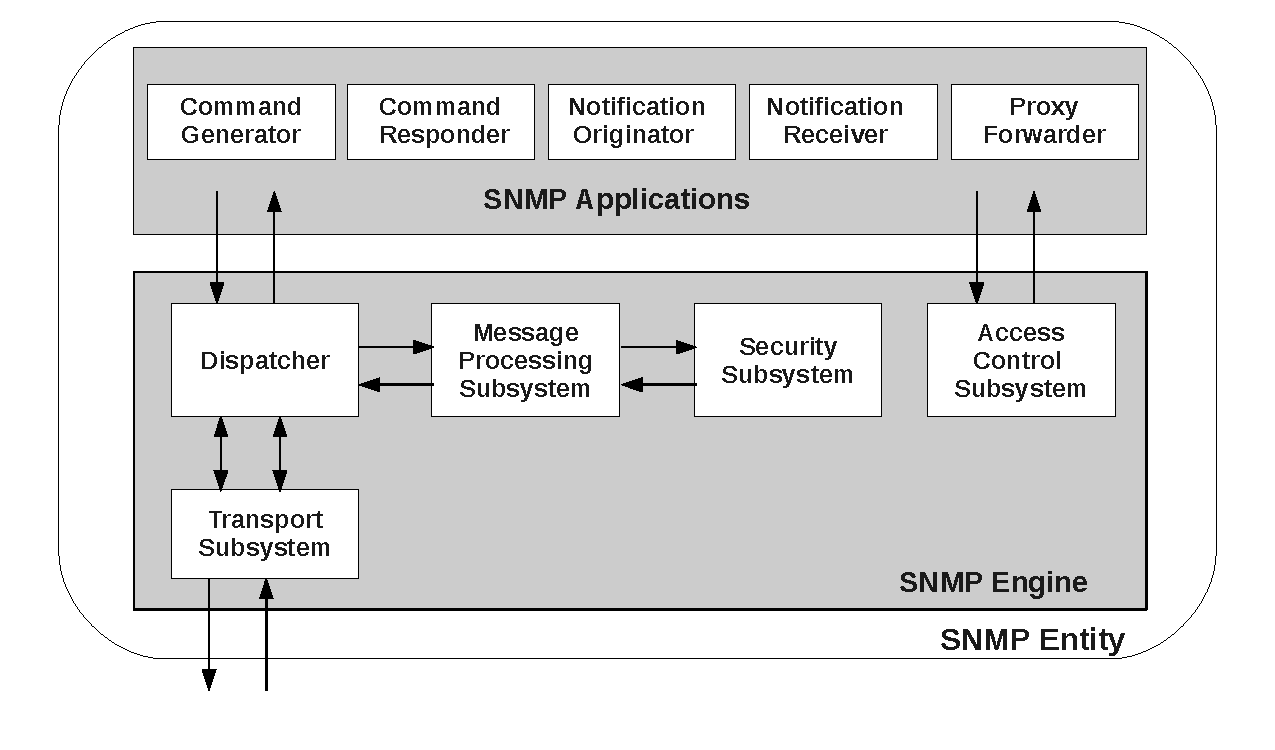
\includegraphics[scale = 0.6]{img/snmp-arch.pdf}
    \caption{Structure of an SNMP entity}   
	\label{fig:snmparch}
\end{center}
\end{figure}

\section{SNMP Operations}

\section{Security Models}

